\section{性能考量}
并行程序的执行速度可能会根据程序的资源需求和硬件的资源限制之间的相互作用而有很大差异。 
管理并行代码和硬件资源限制之间的交互对于在几乎所有并行编程模型中实现高性能非常重要。 
这是一项实用技能,需要深入了解硬件架构,最好通过在专为高性能而设计的并行编程模型中进行实践练习来学习。

到目前为止,我们已经了解了 GPU 架构的各个方面及其对性能的影响。 
在第 4 章“计算架构和调度”中,我们了解了 GPU 的计算架构以及相关的性能考虑因素,例如控制发散和占用。 
在第5章“内存架构和数据局部性”中,我们了解了GPU的片上内存架构以及使用共享内存平铺来实现更多的数据重用。 
在本章中,我们将简要介绍片外内存(DRAM)架构,并讨论相关的性能考虑因素,例如内存合并和内存延迟隐藏。 
然后,我们讨论一种重要的优化类型——线程粒度粗化——它可能针对架构的任何不同方面,具体取决于应用程序。 
最后,我们用一个常见性能优化清单来总结本书的这一部分,该清单将作为优化并行模式性能的指南,
并行模式的性能将在本书的第二部分和第三部分中讨论。

在不同的应用中,不同的架构约束可能占主导地位并成为性能的限制因素,通常称为瓶颈。 
通过将一种资源使用换成另一种资源使用,通常可以显着提高特定 CUDA 设备上应用程序的性能。 
如果由此减轻的资源约束在应用该策略之前是主要约束,并且由此加剧的约束不会对并行执行产生负面影响,则该策略效果很好。 
如果没有这样的理解,性能调整就只是猜测。 合理的策略可能会也可能不会导致性能提升。

\subsection{内存合并}
CUDA 内核性能最重要的因素之一是访问全局内存中的数据,而全局内存的有限带宽可能成为瓶颈。 
CUDA 应用程序广泛利用数据并行性。 当然,CUDA 应用程序往往会在短时间内处理来自全局内存的大量数据,
在第 5 章“内存架构和数据局部性”中,我们研究了利用共享内存来减少数据总量的平铺技术。 
必须由每个线程块中的线程集合从全局内存访问。 在本章中,我们将进一步讨论内存合并技术,
用于以有效的方式在全局内存和共享内存或寄存器之间移动数据。 
内存合并技术通常与切片技术结合使用,以允许 CUDA 设备通过有效利用全局内存带宽来发挥其性能潜力
\footnote{最近的 CUDA 设备使用片上缓存来存储全局内存数据。 
此类缓存会自动合并更多内核访问模式,并在一定程度上减少程序员手动重新安排其访问模式的需要。 
然而,即使有了缓存,合并技术在可预见的将来仍将继续对内核执行性能产生重大影响。}。

\begin{remark}[为什么 DRAM 这么慢?]
下图显示了 DRAM 单元以及访问其内容的路径。 解码器是一种电子电路,使用晶体管驱动连接到数千个单元出口门的线路。 
线路可能需要很长时间才能完全充电或放电到所需的水平。

\begin{figure}[H]
	\centering
	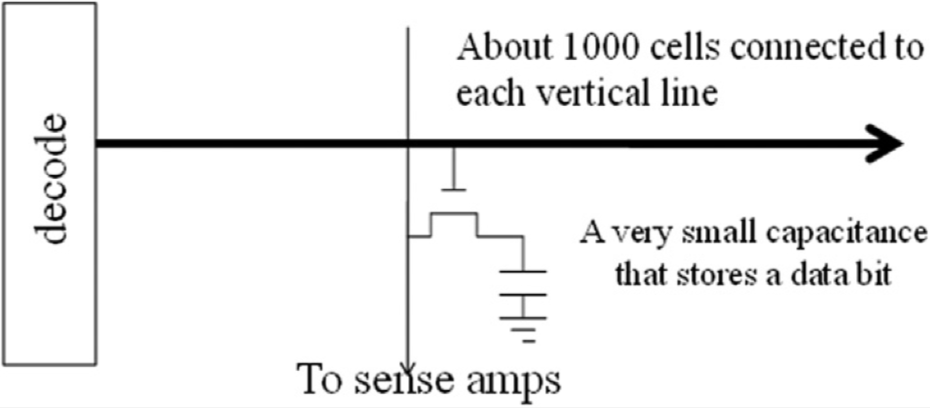
\includegraphics[width=0.9\textwidth]{figs/F6-a.1.png}
\end{figure}

对于单元来说,更艰巨的挑战是驱动垂直线到读出放大器并允许读出放大器检测其内容。 
这是基于电荷共享。 栅极释放出细胞中存储的微量电荷。 
如果单元内容为“1”,那么微量的电荷必须将长位线的大电容的电势提高到足够高的水平,以便能够触发读出放大器的检测机制。 
一个很好的类比是,某人在长长的走廊的一端拿着一小杯咖啡,而在走廊的另一端的人则利用沿着走廊传播的香气来确定咖啡的味道。

人们可以通过在每个单元中使用更大、更强的电容器来加速这一过程。 然而,DRAM 一直在朝着相反的方向发展。 
每个单元中的电容器的尺寸都在稳步减小,因此它们的强度随着时间的推移而降低,以便每个芯片中可以存储更多的位。 
这就是 DRAM 的访问延迟并没有随着时间的推移而减少的原因。
\end{remark}

CUDA设备的全局存储器是用DRAM实现的。 数据位存储在小电容器 DRAM 单元中,其中是否存在微量电荷可区分 1 和 0 值。 
从 DRAM 单元读取数据需要小电容器使用其微小的电荷来驱动通向传感器的高电容线,并启动传感器的检测机制,
该机制确定电容器中是否存在足够的电荷量,以符合 “1。” 在现代 DRAM 芯片中,
这个过程需要数十纳秒(请参阅“为什么 DRAM 如此慢?”边栏)。 这与现代计算设备的亚纳秒时钟周期时间形成鲜明对比。 
由于此过程相对于所需的数据访问速度(每字节亚纳秒访问)非常慢,
因此现代 DRAM 设计使用并行性来提高数据访问速率,通常称为内存访问吞吐量。

每次访问 DRAM 位置时,都会访问包括所请求位置的一系列连续位置。 
每个 DRAM 芯片中都提供了许多传感器,并且它们都并行工作。 每个都感测这些连续位置内的一位的内容。 
一旦被传感器检测到,来自所有这些连续位置的数据就可以高速传输到处理器。 这些访问和传送的连续位置称为 DRAM 突发。 
如果应用程序集中使用来自这些突发的数据,那么 DRAM 可以以比访问真正随机的位置序列的情况高得多的速率提供数据。

认识到现代 DRAM 的突发组织,当前的 CUDA 设备采用了一种技术,
允许程序员通过将线程的内存访问组织成有利的模式来实现高全局内存访问效率。 
该技术利用了线程束中的线程在任何给定时间点执行相同指令的事实。 当 warp 中的所有线程执行加载指令时,
硬件会检测它们是否访问连续的全局内存位置。 换句话说,当线程束中的所有线程访问连续的全局内存位置时,
可以实现最有利的访问模式。 在这种情况下,硬件将所有这些访问组合或合并为对连续 DRAM 位置的合并访问。 
例如,对于给定的 warp 加载指令,如果线程 0 访问全局内存位置 X,线程 1 访问位置 X + 1,线程 2 访问位置 X + 2,
依此类推,所有这些访问将被合并或组合。 访问 DRAM 时将其转换为对连续位置的单个请求
\footnote{不同的CUDA设备还可能对全局内存地址X施加对齐要求。例如,在一些CUDA设备中,X需要与16字(即64字节)边界对齐。 
即X的低六位应全部为0位。 由于二级缓存的存在,这种对齐要求在最近的 CUDA 设备中已经放宽。}。
这种合并访问允许 DRAM 以突发方式传送数据。
\footnote{请注意,现代 CPU 还可以识别其缓存设计中的 DRAM 突发组织。 CPU 高速缓存行通常映射到一个或多个 DRAM 突发。 
充分利用它们所接触的每个缓存行中的字节的应用程序往往比随机访问内存位置的应用程序获得更高的性能。 
我们在本章中介绍的技术可以用来帮助 CPU 程序实现高性能。}。

\begin{figure}[H]
	\centering
	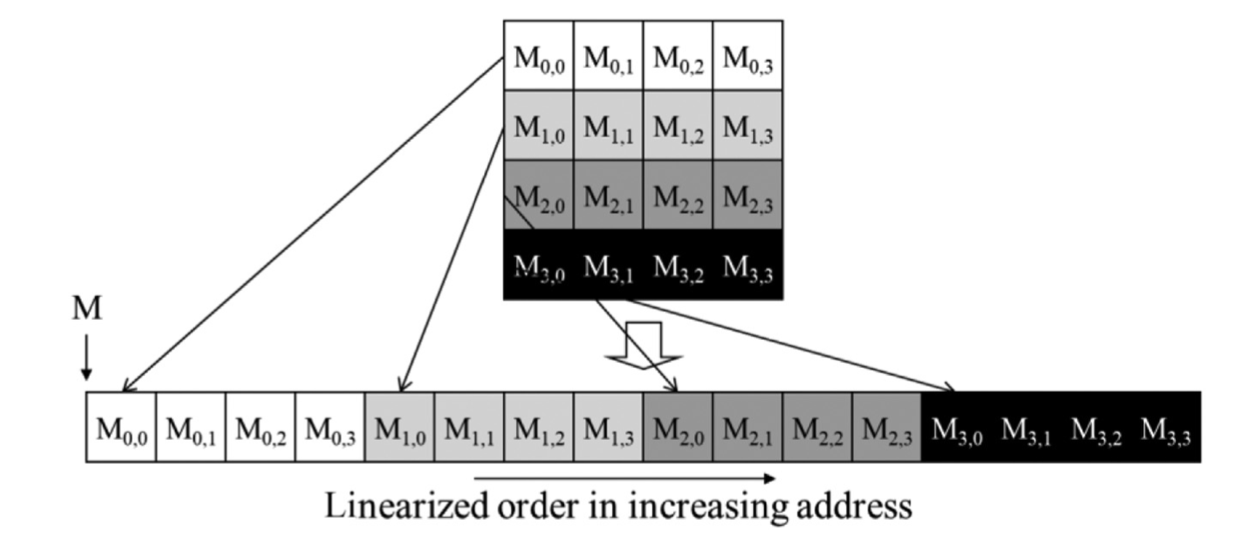
\includegraphics[width=0.9\textwidth]{figs/F6.1.png}
	\caption{\textit{根据行优先顺序将矩阵元素放入线性数组中。}}
\end{figure}

为了理解如何有效地使用合并硬件,我们需要回顾一下在访问 C 多维数组元素时内存地址是如何形成的。 
回想一下第 3 章“多维网格和数据”(为了方便起见,图 3.3 在此复制为图 6.1),
C 和 CUDA 中的多维数组元素根据行优先约定放置到线性寻址内存空间中。 
回想一下,术语行优先指的是数据的放置保留了行的结构:行中的所有相邻元素都被放置到地址空间中的连续位置。 
在图 6.1 中,第 0 行的四个元素首先按照它们在该行中出现的顺序放置。 然后放置第 1 行中的元素,然后是第 2 行的元素,
最后是第 3 行的元素。应该清楚的是,$M_{0,0}$ 和 $M_{1,0}$ 尽管在二维矩阵中看起来是连续的,
但它们是 在线性寻址存储器中分开放置四个位置。

\begin{figure}[H]
	\centering
	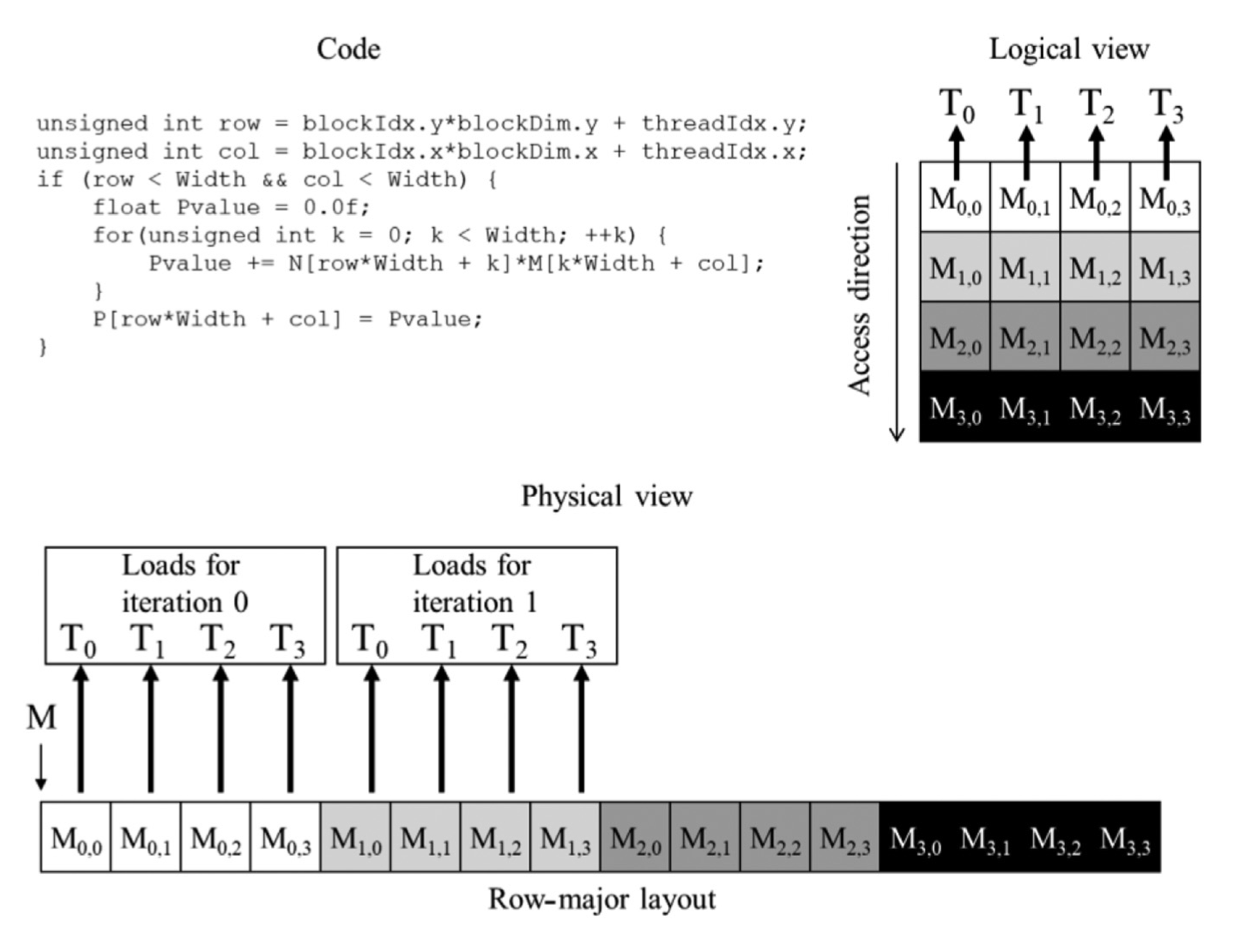
\includegraphics[width=0.9\textwidth]{figs/F6.2.png}
	\caption{\textit{合并访问模式。}}
\end{figure}

假设图 6.1 中的多维数组是一个矩阵,在矩阵乘法中用作第二个输入矩阵。 
在这种情况下,warp 中分配给连续输出元素的连续线程将迭代该输入矩阵的连续列。 
图 6.2 的左上部分显示了此计算的代码,右上部分显示了访问模式的逻辑视图:连续的线程迭代连续的列。 
通过检查代码可以看出对 M 的访问可以合并。 数组 M 的索引为 k × Width+col。 
变量 k 和 Width 在经纱中的所有线程中具有相同的值。 变量 col 定义为 blockIdx。 x * blockDim.x+threadIdx.x,
这意味着连续的线程(具有连续的 threadIdx.x 值)将具有连续的 col 值,因此将访问 M 的连续元素。

图 6.2 的底部显示了访问模式的物理视图。 在迭代 0 中,连续线程将访问内存中相邻的第 0 行中的连续元素,
如图 6.2 中的“迭代 0 的负载”所示。 在迭代 1 中,连续线程将访问第 1 行中在内存中也相邻的连续元素,
如图 6.2 中的“迭代 1 的负载”所示。 此过程对所有行都持续进行。 
正如我们所看到的,在此过程中线程形成的内存访问模式是一种可以合并的有利模式。 
事实上,在我们迄今为止实现的所有内核中,我们的内存访问都是自然合并的。

现在假设矩阵按列优先顺序而不是行优先顺序存储。 造成这种情况的原因可能有多种。 
例如,我们可能会乘以以行优先顺序存储的矩阵的转置。 在线性代数中,我们经常需要使用矩阵的原始形式和转置形式。 
最好避免创建和存储这两种表单。 常见的做法是以一种形式(例如原始形式)创建矩阵。 
当需要转置形式时,可以通过切换行索引和列索引的角色来访问原始形式来访问其元素。 
在 C 中,这相当于将转置矩阵视为原始矩阵的列优先布局。 
不管出于什么原因,让我们观察一下当矩阵乘法示例的第二个输入矩阵以列优先顺序存储时所实现的内存访问模式。

\begin{figure}[H]
	\centering
	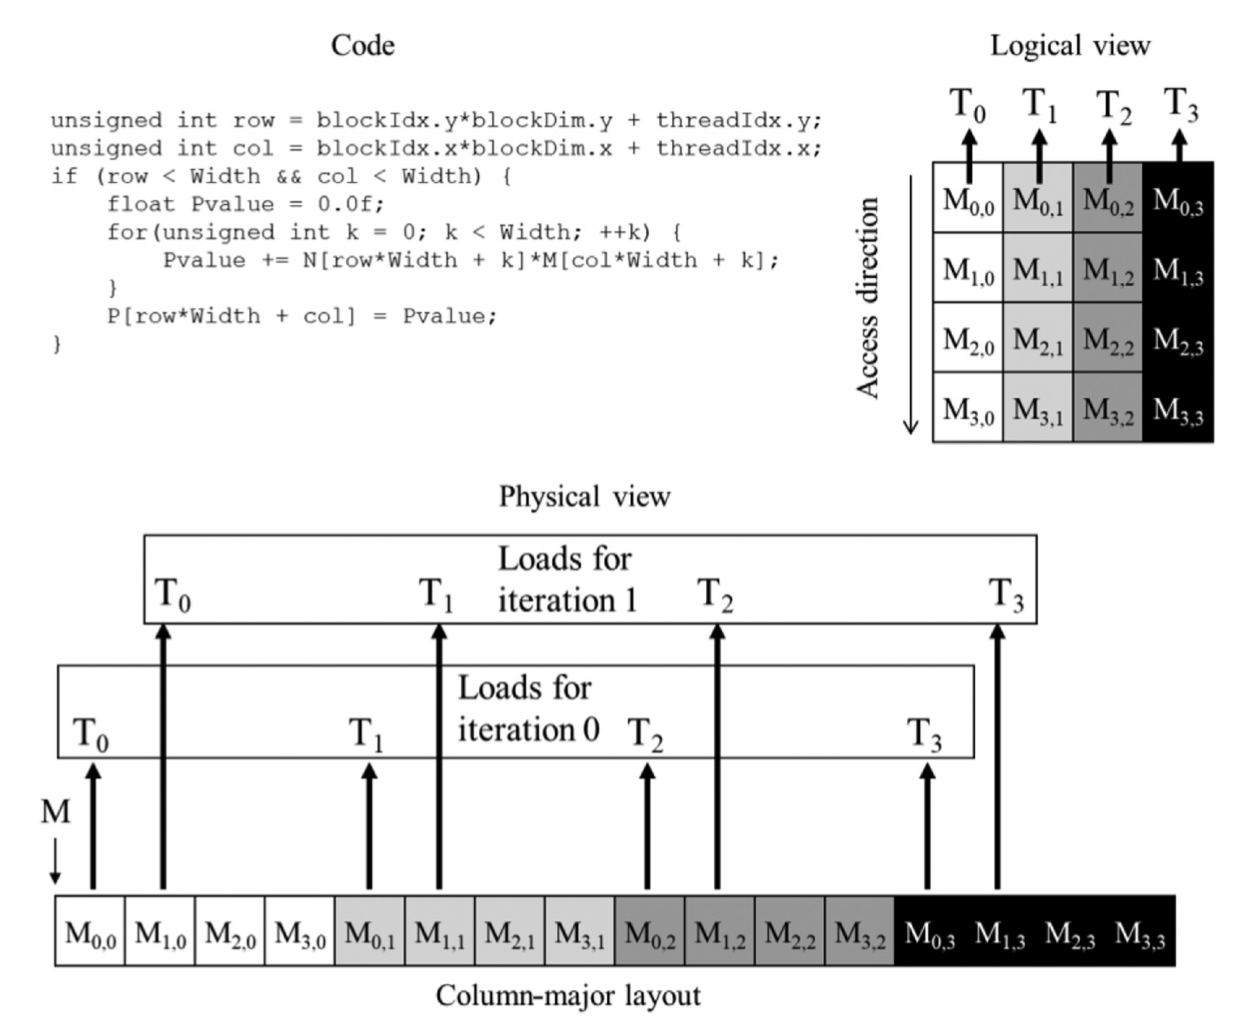
\includegraphics[width=0.9\textwidth]{figs/F6.3.png}
	\caption{\textit{未合并的访问模式。}}
\end{figure}

图 6.3 说明了当矩阵按列优先顺序存储时,连续线程如何迭代连续列。 
图6.3的左上部分显示了代码,右上部分显示了存储器访问的逻辑视图。 该程序仍在尝试让每个线程访问矩阵 M 的一列。
通过检查代码可以看出对 M 的访问不利于合并。 数组 M 的索引是 col × Width+k。 
和之前一样,col 定义为 blockIdx.x * blockDim.x+threadIdx.x,
这意味着连续的线程(具有连续的 threadIdx.x 值)将具有连续的 col 值。 
然而,在 M 的索引中,col 乘以 Width,这意味着连续的线程将访问 M 中相隔 Width 的元素。 因此,这些访问不利于合并。

在图6.3的底部,我们可以看到内存访问的物理视图与图6.2有很大不同。 
在迭代 0 中,连续线程将逻辑上访问第 0 行中的连续元素,但这次由于列优先布局,它们在内存中不相邻。 
这些载荷在图 6.3 中显示为“迭代 0 的载荷”。 类似地,在迭代 1 中,连续线程将访问第 1 行中在内存中也不相邻的连续元素。 
对于实际矩阵,每个维度通常有数百甚至数千个元素。 相邻线程在每次迭代中访问的 M 个元素可以相距数百甚至数千个元素。 
硬件将确定对这些元素的访问彼此相距较远并且无法合并。

当计算自然不适合时,可以采用多种策略来优化代码以实现内存合并。 
一种策略是重新安排线程与数据的映射方式; 另一种策略是重新排列数据本身的布局。 
我们将在第 6.4 节中讨论这些策略,并在本书中查看如何应用它们的示例。 
另一种策略是以合并的方式在全局内存和共享内存之间传输数据,并在共享内存中执行不利的访问模式,这提供了更快的访问延迟。 
我们还将在本书中看到使用此策略的示例优化,包括我们现在将应用于矩阵-矩阵乘法的优化,其中第二个输入矩阵采用列主布局。 
这种优化称为转角。

\begin{figure}[H]
	\centering
	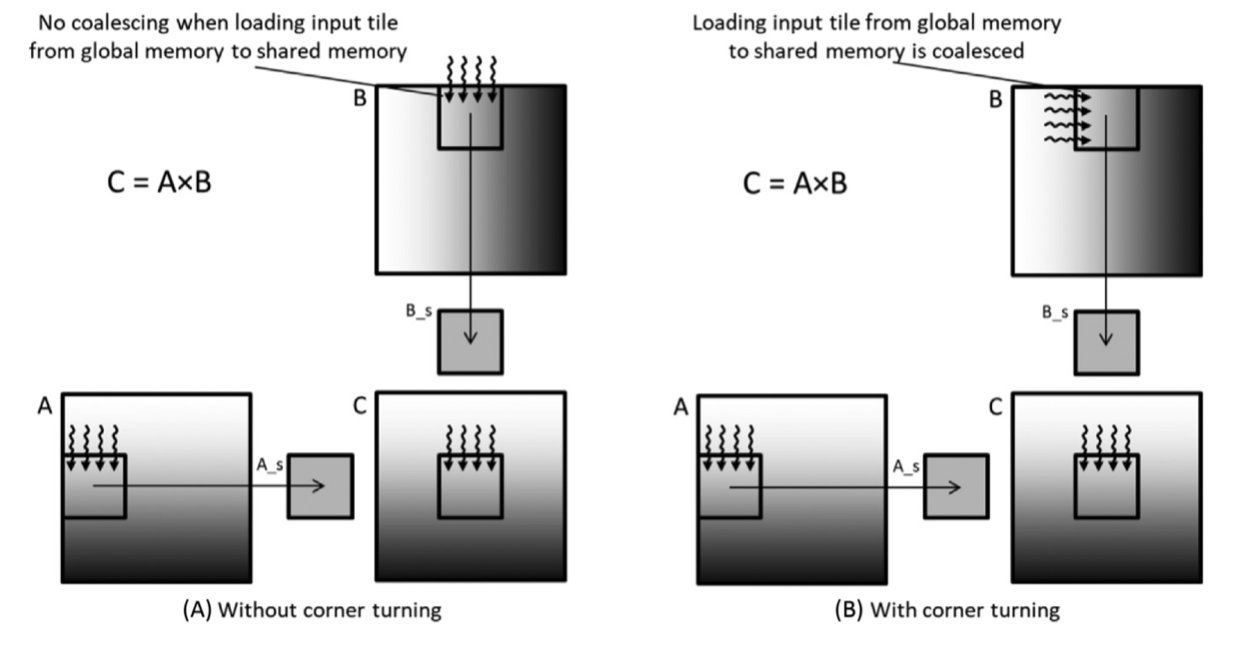
\includegraphics[width=0.9\textwidth]{figs/F6.4.png}
	\caption{\textit{应用转角来合并对矩阵 B 的访问,该矩阵以列优先布局存储。}}
\end{figure}

图 6.4 说明了如何应用转角的示例。 在此示例中,A 是在全局内存中以行优先布局存储的输入矩阵,
B 是在全局内存中以列优先布局存储的输入矩阵。 它们相乘产生一个输出矩阵 C,该矩阵以行优先布局存储在全局内存中。 
该示例说明了负责输出图块顶部边缘的四个连续元素的四个线程如何加载输入图块元素。

对矩阵 A 中输入块的访问与第 5 章“内存架构和数据局部性”中的类似。 四个线程加载输入图块顶部边缘的四个元素。 
每个线程加载一个输入元素,其输入图块中的本地行索引和列索引与输出图块中线程的输出元素的索引相同。 
这些访问被合并,因为连续的线程根据行优先布局访问 A 的同一行中在内存中相邻的连续元素。

另一方面,对矩阵 B 中输入块的访问需要与第 5 章“内存架构和数据局部性”中的访问不同。 
图 6.4(A) 显示了如果我们使用与第 5 章“内存架构和数据局部性”中相同的安排,访问模式会是什么样子。 
尽管四个线程逻辑上加载输入图块顶部边缘的四个连续元素,但由于 B 元素的列优先布局,
连续线程加载的元素在内存中彼此相距较远。 换句话说,负责输出图块同一行中的连续元素的连续线程加载内存中的非连续位置,
这会导致未合并的内存访问。

这个问题可以通过分配四个连续的线程来加载输入图块中左边缘(同一列)的四个连续元素来解决,如图6.4(B)所示。 
直观上,当每个线程计算用于加载 B 输入图块的线性化索引时,我们正在交换 threadIdx.x 和 threadIdx.y 的角色。 
由于 B 采用列优先布局,因此同一列中的连续元素在内存中是相邻的。 
因此,连续的线程加载内存中相邻的输入元素,这确保了内存访问的合并。 
可以编写代码以将 B 元素的图块以列优先布局或行优先布局放入共享内存中。 
无论哪种方式,在加载输入图块后,每个线程都可以访问其输入,而性能损失很小。 
这是因为共享内存是通过 SRAM 技术实现的,不需要合并。

\begin{figure}[H]
	\centering
	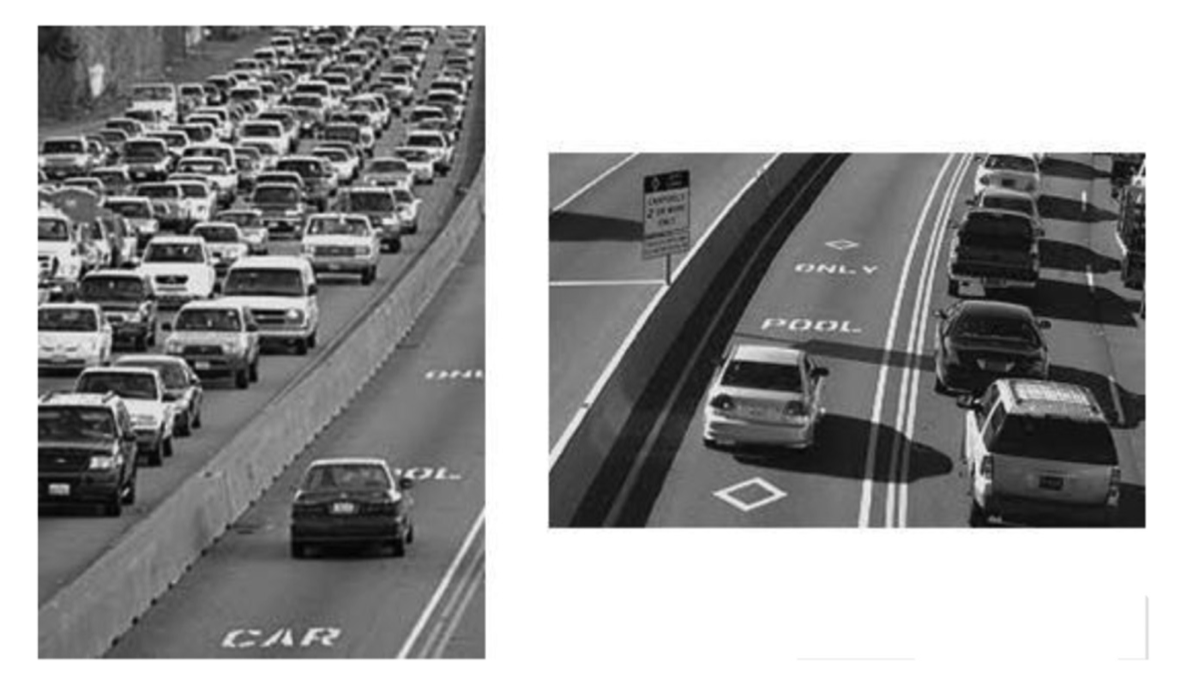
\includegraphics[width=0.9\textwidth]{figs/F6.5.png}
	\caption{\textit{减少高速公路系统的交通拥堵。}}
\end{figure}

内存合并的主要优点是,它通过将多个内存访问合并为一次访问来减少全局内存流量。 
当同时发生并访问相邻的存储位置时,可以组合访问。 交通拥堵不仅仅出现在计算领域。 
我们大多数人都经历过高速公路系统的交通拥堵,如图 6.5 所示。 高速公路交通拥堵的根本原因是,
太多的汽车试图在一条为车辆数量少得多的道路上行驶。 当拥堵发生时,每辆车的行驶时间会大大增加。 
当交通拥堵时,上班时间很容易就会增加一倍或三倍。

大多数减少交通拥堵的解决方案都涉及减少道路上的汽车数量。 假设通勤人数不变,人们需要拼车以减少道路上的汽车数量。 
拼车是一种常见的拼车方式,即一群通勤者的成员轮流驾驶一辆车去上班。 政府通常需要制定鼓励拼车的政策。 
在一些国家,政府只是禁止某些类别的汽车每天上路。 例如,星期一、星期三或星期五可能不允许车牌号为奇数的汽车上路。 
这鼓励了在不同日期允许使用汽车的人组成拼车团体。 在其他国家,政府可能会对减少道路上汽车数量的行为提供激励。 
例如,在某些国家,拥堵高速公路的某些车道被指定为拼车车道; 只有两到三人以上的汽车才允许使用这些车道。 
也有一些国家的政府让汽油变得非常昂贵,以至于人们为了省钱而拼车。 
所有这些鼓励拼车的措施都是为了克服拼车需要额外努力的事实,如图6.6所示。

\begin{figure}[H]
	\centering
	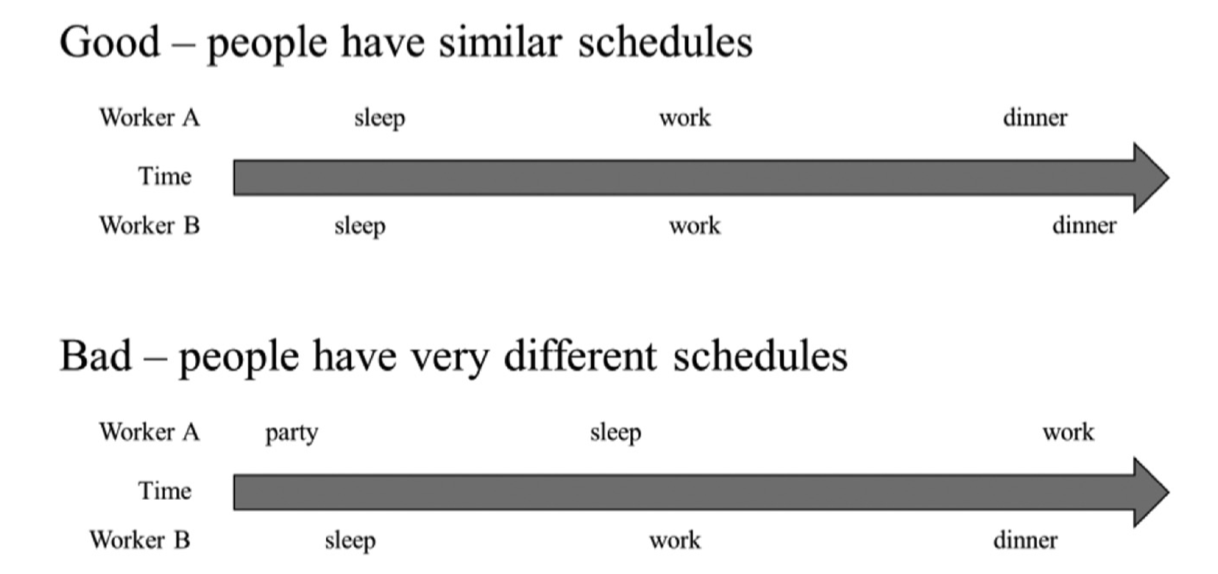
\includegraphics[width=0.9\textwidth]{figs/F6.6.png}
	\caption{\textit{拼车需要人与人之间的同步。}}
\end{figure}

拼车要求希望拼车的工人妥协并就共同的通勤时间表达成一致。 图 6.6 的上半部分显示了良好的拼车时间表模式。 
时间从左向右。 工人 A 和工人 B 的睡眠、工作和晚餐时间表相似。 这使得这两名工人可以轻松地用一辆车上下班和回家。 
他们相似的时间表使他们更容易就共同的出发时间和返回时间达成一致。 图 6.6 下半部分所示的时间表并非如此。 
在本例中,工人 A 和工人 B 的日程安排截然不同。 工人A聚会到天亮,白天睡觉,晚上上班。 
工人B晚上睡觉,早上上班,下午6:00回家吃晚饭。 时间表差异如此之大,以至于这两名工人不可能协调同一时间开车上班和回家。

内存合并与拼车安排非常相似。 我们可以将数据视为通勤者,将 DRAM 访问请求视为车辆。 
当DRAM请求的速率超过DRAM系统规定的访问带宽时,流量拥塞加剧,运算单元变得空闲。 
如果多个线程从同一 DRAM 位置访问数据,它们可能会形成“拼车”并将其访问合并到一个 DRAM 请求中。 
然而,这要求线程具有相似的执行调度,以便它们的数据访问可以合二为一。 
同一 warp 中的线程是完美的候选者,因为它们都通过 SIMD 执行同时执行加载指令。

\subsection{隐藏内存延迟}
\begin{figure}[H]
	\centering
	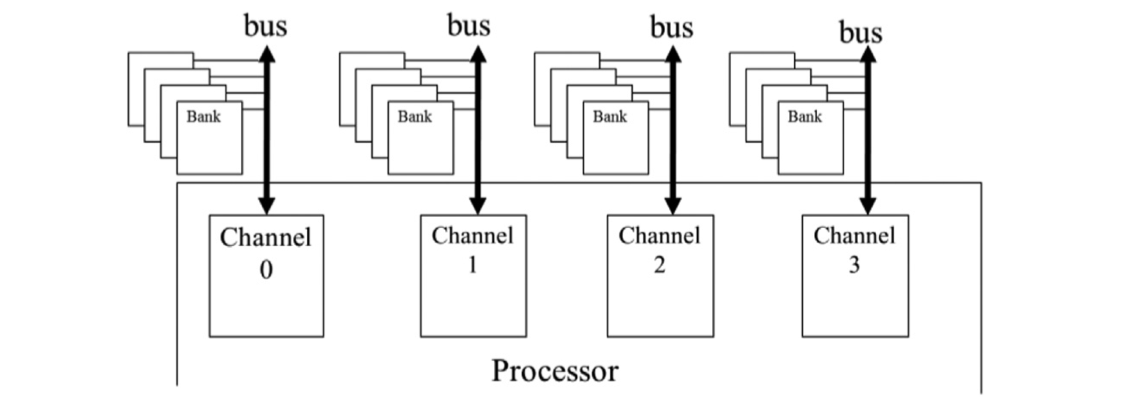
\includegraphics[width=0.9\textwidth]{figs/F6.7.png}
	\caption{\textit{DRAM 系统中的通道和存储体。}}
\end{figure}

正如我们在第 6.1 节中所解释的,DRAM 突发是并行组织的一种形式:并行访问 DRAM 核心阵列中的多个位置。 
然而,仅突发不足以实现现代处理器所需的 DRAM 访问带宽水平。 
DRAM 系统通常采用另外两种形式的并行组织:存储体(banks)和通道(channels)。 
在最高级别,处理器包含一个或多个通道。 每个通道都是一个内存控制器,其总线将一组 DRAM 存储体连接到处理器。 
图 6.7 显示了一个包含四个通道的处理器,每个通道都有一条总线将四个 DRAM 组连接到处理器。 
在实际系统中,处理器通常具有一到八个通道,并且每个通道连接大量组。

总线的数据传输带宽由其宽度和时钟频率定义。 现代双数据速率 (DDR) 总线在每个时钟周期执行两次数据传输:
一次在每个时钟周期的上升沿,一次在下降沿。 例如,时钟频率为1GHz的64位DDR总线,其带宽为8B×2×1GHz=16GB/s。 
这似乎是一个很大的数字,但对于现代 CPU 和 GPU 来说往往太小。 
现代 CPU 可能需要至少 32 GB/s 的内存带宽,而现代 GPU 可能需要 256 GB/s。 
对于此示例,CPU 将需要 2 个通道,GPU 将需要 16 个通道。

\begin{figure}[H]
	\centering
	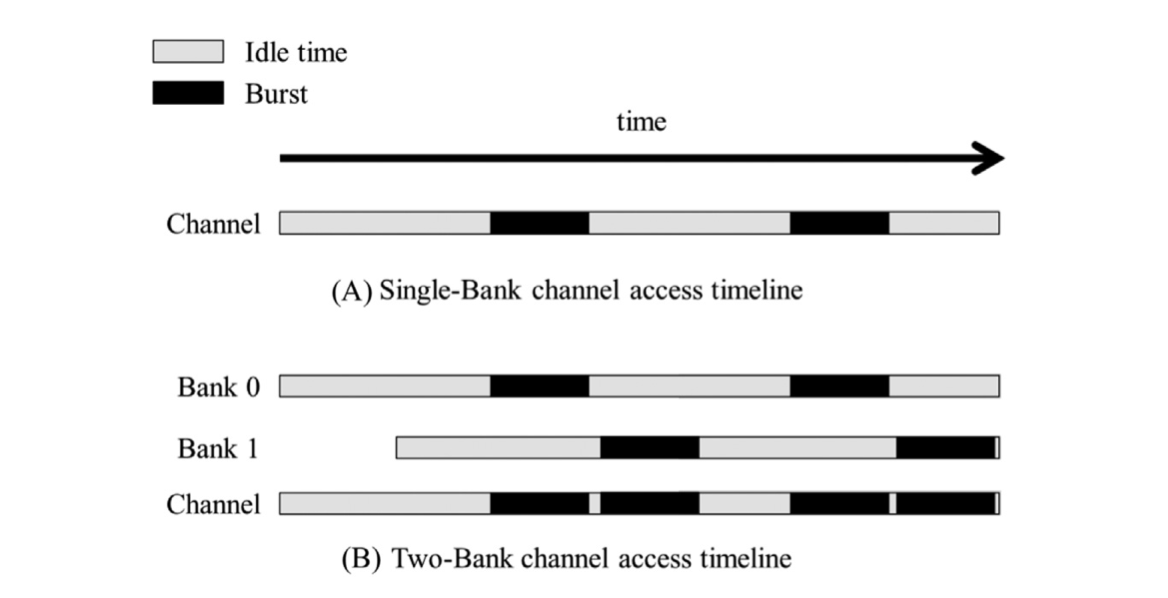
\includegraphics[width=0.9\textwidth]{figs/F6.8.png}
	\caption{\textit{储存体提高了通道数据传输带宽的利用率。}}
\end{figure}

对于每个通道,与其连接的 Bank 数量由充分利用总线数据传输带宽所需的 Bank 数量决定。 如图 6.8 所示。 
每个存储体包含一个 DRAM 单元阵列、用于访问这些单元的传感放大器以及用于将突发数据传送到总线的接口(第 6.1 节)。

图 6.8(A) 说明了单个存储体连接到通道时的数据传输时序。 它显示了对存储体中 DRAM 单元的两次连续内存读取访问的时序。 
回想一下第 6.1 节,每次访问都涉及解码器启用单元以及单元与传感放大器共享其存储的电荷的较长延迟。 
该延迟显示为时间帧左端的灰色部分。 一旦传感放大器完成其工作,突发数据就会通过总线传送。 
通过总线传输突发数据的时间如图 6.8 中时间帧的左侧黑色部分所示。 
在传输突发数据(右侧的黑色部分)之前,第二次存储器读取访问将产生类似的长访问延迟(时间帧的黑色部分之间的灰色部分)。

实际上,访问延迟(灰色部分)比数据传输时间(黑色部分)长得多。 
显然,单组组织的访问传输时序将严重未充分利用通道总线的数据传输带宽。 
例如,如果DRAM单元阵列访问延迟与数据传输时间的比率为20:1,则通道总线的最大利用率将为1/21=4.8\%; 
也就是说,16 GB/s 通道将以不超过 0.76 GB/s 的速率向处理器传送数据。 
这是完全不能接受的。 通过将多个存储体连接到通道总线来解决这个问题。

当两个存储体连接到通道总线时,可以在第二个存储体中发起访问,而第一个存储体正在服务另一个访问。 
因此,可以重叠访问 DRAM 单元阵列的延迟。 图 6.8(B) 显示了两个存储体组织的时序。 
我们假设组 0 的启动时间早于图 6.8 所示的窗口。 在第一个存储体开始访问其单元阵列后不久,
第二个存储体也开始访问其单元阵列。 当存储体 0 中的访问完成时,它会传输突发数据(时间帧最左边的黑暗部分)。 
一旦存储体 0 完成其数据传输,存储体 1 就可以传输其突发数据(第二个暗部分)。 下次访问时会重复此模式。

从图 6.8(B) 中,我们可以看到,通过拥有两个存储体,我们有可能使通道总线的数据传输带宽利用率加倍。 
一般来说,如果单元阵列访问延迟与数据传输时间的比率为R,则如果我们希望充分利用通道总线的数据传输带宽,
则至少需要R + 1个bank。 例如,如果比率为 20,则我们将需要至少 21 个组连接到每个通道总线。 
一般来说,连接到每个通道总线的组数量需要大于 R,原因有两个。 
一是拥有更多的储存体会降低针对同一储存体的多个同时访问的可能性,这种现象称为储存体冲突。 
由于每个存储体一次只能服务一次访问,因此单元阵列访问延迟对于这些冲突的访问不再重叠。 
拥有更多的储存体会增加这些访问分布在多个储存体之间的可能性。 
第二个原因是每个单元阵列的大小被设置为实现合理的延迟和可制造性。 这限制了每个储存体可以提供的单元数量。 
人们可能需要许多存储体才能支持所需的内存大小。

线程的并行执行与DRAM系统的并行组织之间存在着重要的联系。 
为了达到设备指定的内存访问带宽,必须有足够数量的线程同时进行内存访问。 
这一观察反映了最大化占有率的另一个好处。 
回想一下,在第 4 章“计算架构和调度”中,我们看到最大化占用率可确保流式多处理器 (SM) 上驻留足够的线程来隐藏核心管道延迟,
从而有效地利用指令吞吐量。 正如我们现在所看到的,最大化占用率还具有额外的好处,
即确保发出足够的内存访问请求来隐藏 DRAM 访问延迟,从而有效地利用内存带宽。 
当然,为了实现最佳的带宽利用率,这些内存访问必须均匀分布在通道和存储体上,并且对存储体的每次访问也必须是合并访问。

\begin{figure}[H]
	\centering
	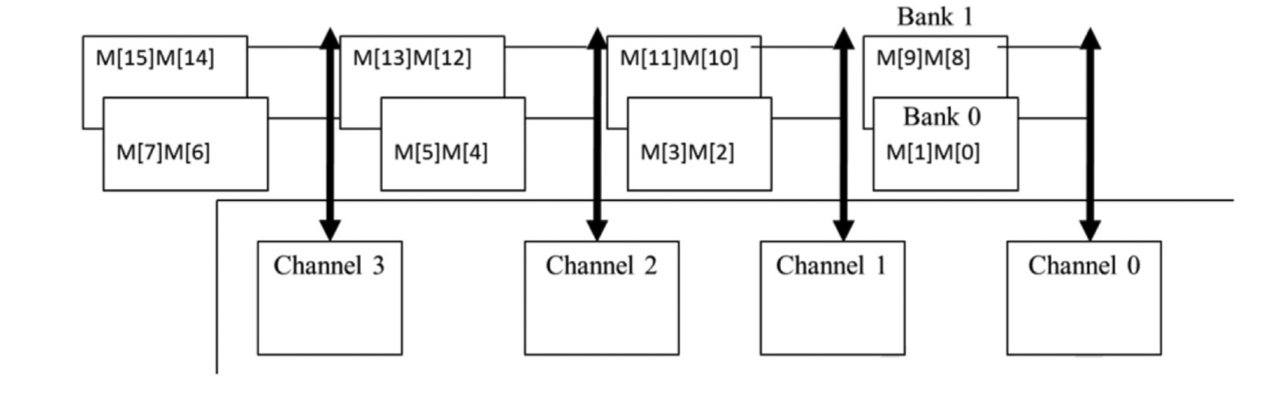
\includegraphics[width=0.9\textwidth]{figs/F6.9.png}
	\caption{\textit{将数组元素分配到通道和储存体中。}}
\end{figure}

图 6.9 显示了将数组 M 的元素分配到通道和组的玩具示例。 我们假设两个元素(8 字节)的小突发大小。 
分发是通过硬件设计完成的。 通道和后端的寻址使得数组的前 8 个字节(M[0] 和 M[1])存储在通道 0 的存储体 0 中,
接下来的 8 个字节(M[2] 和 M[3] ]) 在通道 1 的存储体 0 中,
接下来的 8 个字节(M[4] 和 M[5])在通道 2 的存储体 0 中,
以及接下来的 8 个字节(M[6] 和 M[7])在通道 3 的存储体 0 中。

此时,分配回绕到通道 0,但将使用存储体 1 来存储接下来的 8 个字节(M[8] 和 M[9])。 
因此,元素 M[10] 和 M[11] 将位于通道 1 的 Bank 1 中,
M[12] 和 M[13] 将位于通道 2 的 Bank 1 中,M[14] 和 M[15] 将位于 在通道 3 的存储体 1 中。
虽然图中未显示,但任何附加元素都将被环绕并从通道 0 的存储体 0 开始。
例如,如果有更多元素,则 M[16] 和 M[17] 将 存储在通道 0 的 Bank 0 中,
M[18] 和 M[19] 将存储在通道 1 的 Bank 0 中,以此类推。

图 6.9 所示的分配方案通常称为交错数据分配,将元素分布在系统中的存储体和通道中。 
该方案确保即使是相对较小的阵列也能很好地分布。 因此,我们只分配足够的元素来充分利用通道 0 的存储体 0 的 DRAM 突发,
然后再转移到通道 1 的存储体 0。
在我们的玩具示例中,只要我们至少有 16 个元素,分配就会涉及所有通道 以及用于存储元素的储存体。

\begin{figure}[H]
	\centering
	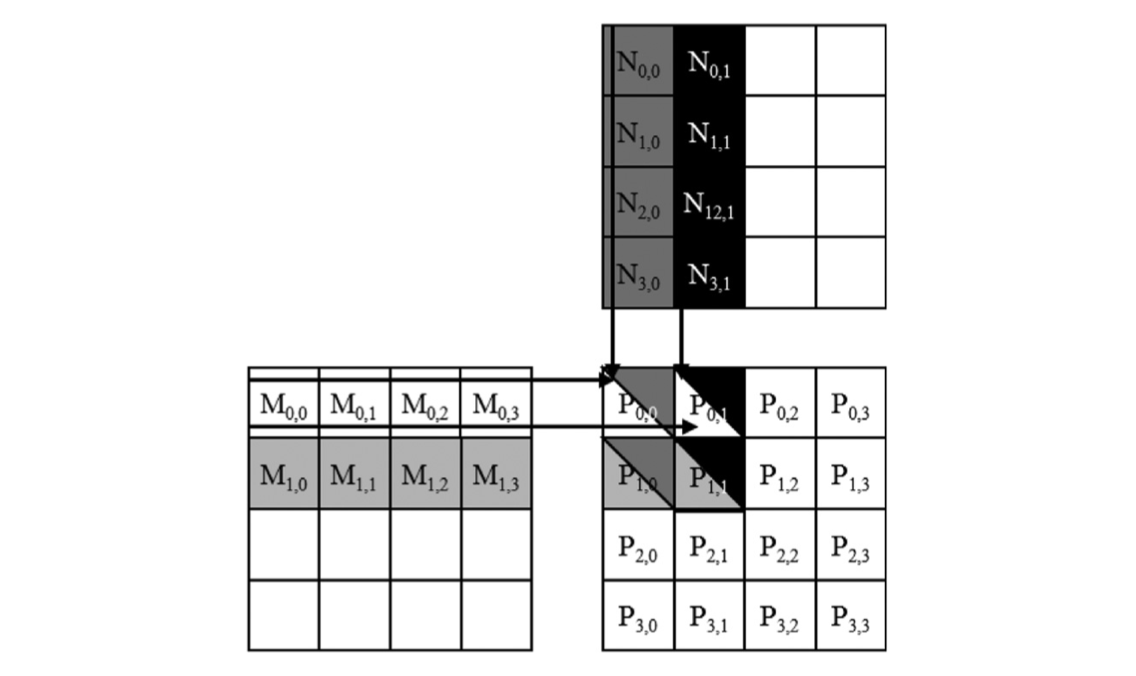
\includegraphics[width=0.9\textwidth]{figs/F6.10.png}
	\caption{\textit{矩阵乘法的一个小例子(从图 5.5 复制)。}}
\end{figure}

我们现在说明并行线程执行和并行内存组织之间的交互。 我们将使用图 5.5 中的示例,复制为图 6.10。 
我们假设乘法将使用 $2 \times 2$ 个线程块和 $2 \times 2$ 个图块来执行。

\begin{figure}[H]
	\centering
	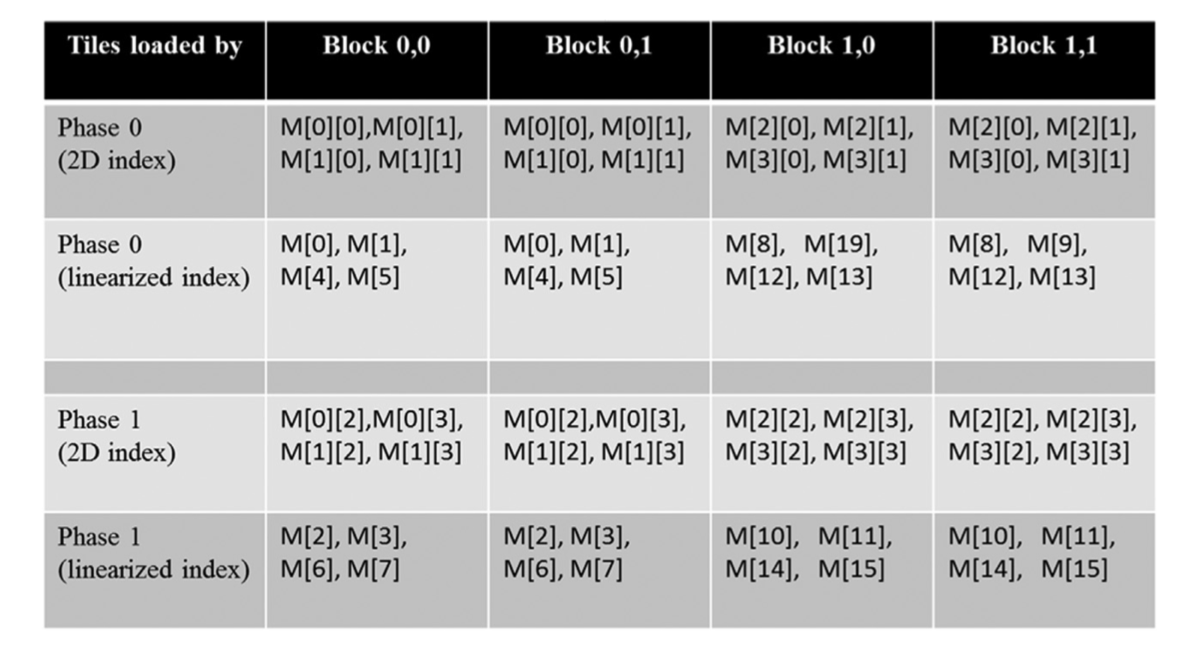
\includegraphics[width=0.9\textwidth]{figs/F6.11.png}
	\caption{\textit{每个阶段由线程块加载 M 个元素。}}
\end{figure}

在内核执行的阶段 0 期间,所有四个线程块都将加载它们的第一个图块。 每个图块涉及的M个元素如图6.11所示。 
第 2 行显示了在第 0 阶段访问的 M 个元素及其 2D 索引。 第 3 行显示相同的 M 元素及其线性化索引。 
假设所有线程块都是并行执行的。 我们看到每个块都会进行两次合并访问。

根据图 6.9 中的分布,这些合并访问将针对通道 0 中的两个存储体以及通道 2 中的两个存储体进行。
这四个访问将并行进行,以充分利用两个通道并改善 每个通道的数据传输带宽的利用率。

我们还看到 $block_{0,0}$ 和 $block_{0,1}$ 将加载相同的 M 元素。 
大多数现代设备都配备了缓存,只要这些块的执行时间彼此足够接近,缓存就会将这些访问合并为一个。 
事实上,GPU设备中的高速缓冲存储器主要是为了组合此类访问而设计的,并减少对DRAM系统的访问次数。

第 4 行和第 5 行显示了在内核执行的第 1 阶段加载的 M 元素。 我们看到现在对通道 1 和通道 3 中的存储体进行访问。
这些访问将再次并行完成。 读者应该清楚,线程的并行执行和DRAM系统的并行结构之间存在共生关系。 
一方面,要充分利用DRAM系统的潜在访问带宽,需要许多线程同时访问DRAM中的数据。 
另一方面,设备的执行吞吐量依赖于对DRAM系统并行结构(即存储体和通道)的良好利用。 
例如,如果同时执行的线程都访问同一通道中的数据,则内存访问吞吐量和整体设备执行速度将大大降低。

请读者验证将两个较大的矩阵(例如 $8 \times 8$ 与相同的 $2 \times 2$ 线程块配置)相乘将利用图 6.9 中的所有四个通道。 
另一方面,增加的 DRAM 突发大小将需要乘以更大的矩阵,以充分利用所有通道的数据传输带宽。

\subsection{线程粗化}
到目前为止,在我们见过的所有内核中,工作都以最细粒度跨线程并行化。 也就是说,每个线程都被分配了尽可能小的工作单元。 
例如,在向量加法内核中,每个线程都被分配一个输出元素。 
在 RGB 到灰度转换和图像模糊内核中,每个线程在输出图像中分配一个像素。 
在矩阵乘法内核中,每个线程都被分配了输出矩阵中的一个元素。

以最细粒度跨线程并行化工作的优点是,它增强了透明的可扩展性,如第 4 章“计算架构和调度”中所述。 
如果硬件有足够的资源来并行执行所有工作,那么应用程序就已经暴露了足够的并行性来充分利用硬件。 
否则,如果硬件没有足够的资源来并行执行所有工作,则硬件可以通过一个接一个地执行线程块来简单地串行化工作。

当并行化工作需要付出“代价”时,以最细粒度并行化工作的缺点就会出现。 
这种并行性的代价可以有多种形式,例如不同线程块的数据冗余加载、冗余工作、同步开销等。 
当线程由硬件并行执行时,这种并行性的代价通常是值得付出的。 
然而,如果硬件由于资源不足而最终将工作串行化,那么这个代价就不必要地付出了。 
在这种情况下,程序员最好部分串行化工作并减少并行性所付出的代价。 
这可以通过为每个线程分配多个工作单元来完成,这通常称为线程粗化。

\begin{figure}[H]
	\centering
	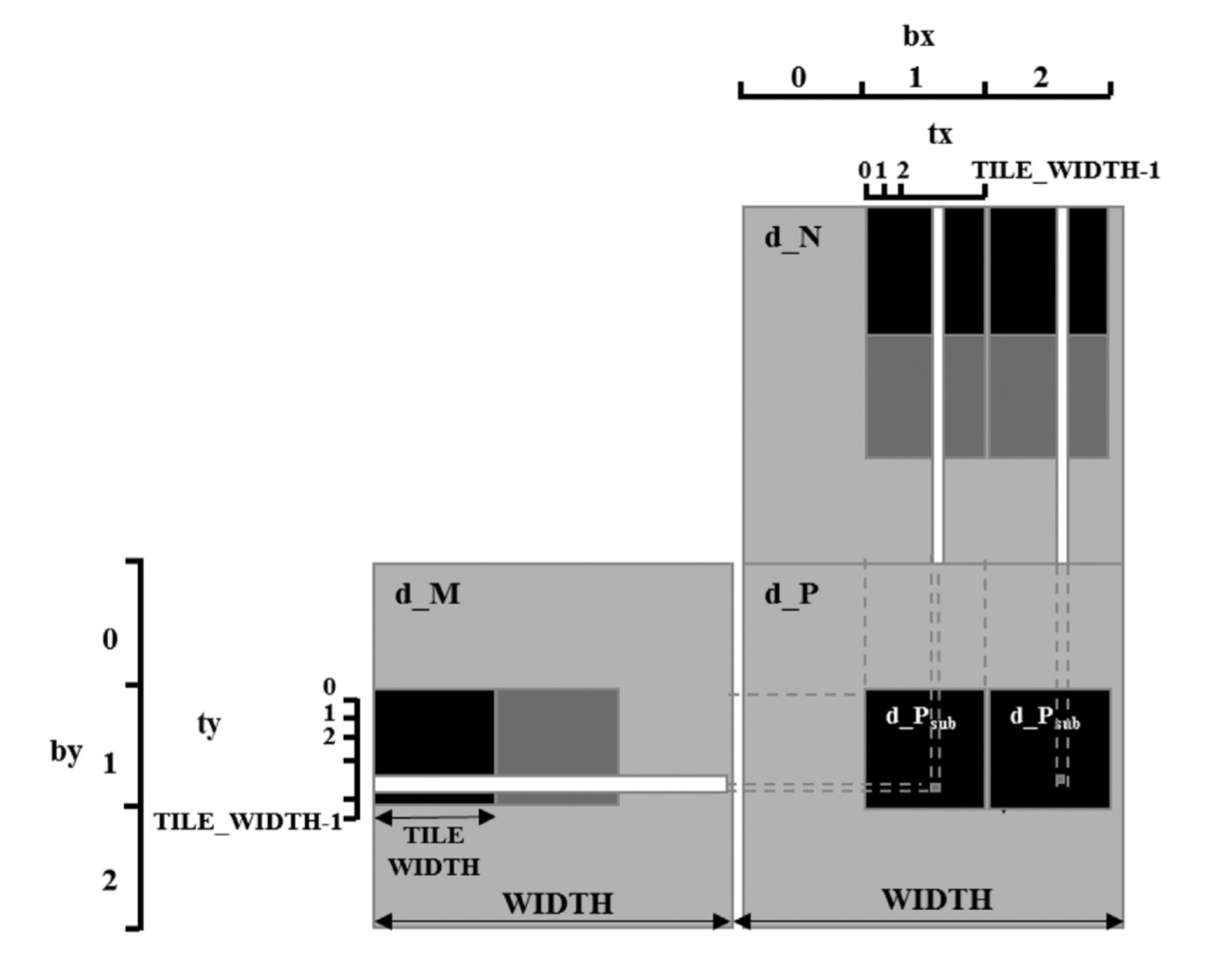
\includegraphics[width=0.9\textwidth]{figs/F6.12.png}
	\caption{\textit{用于平铺矩阵乘法的线程粗化。}}
\end{figure}

我们使用第 5 章“内存架构和数据局部性”中的平铺矩阵乘法示例演示了线程粗化优化。 
图 6.12 描述了计算输出矩阵 P 的两个水平相邻输出块的存储器访问模式。
对于这些输出块中的每一个,我们观察到需要加载矩阵 N 的不同输入块。 然而,为两个输出图块加载矩阵 M 的相同输入图块。

在第 5 章“内存架构和数据局部性”的分片实现中,每个输出分片由不同的线程块处理。 
由于共享内存内容不能跨块共享,因此每个块必须加载自己的矩阵 M 输入图块副本。
虽然让不同的线程块加载相同的输入图块是多余的,但这是我们为了能够 使用不同的块并行处理两个输出图块。 
如果这些线程块并行运行,这个代价可能是值得的。 另一方面,如果这些线程块被硬件串行化,那么付出的代价就是白白的。 
在后一种情况下,程序员最好让单个线程块处理两个输出图块,从而块中的每个线程处理两个输出元素。 
这样,粗化的线程块将加载 M 的输入图块一次并将它们重新用于多个输出图块。

\begin{figure}[H]
	\centering
	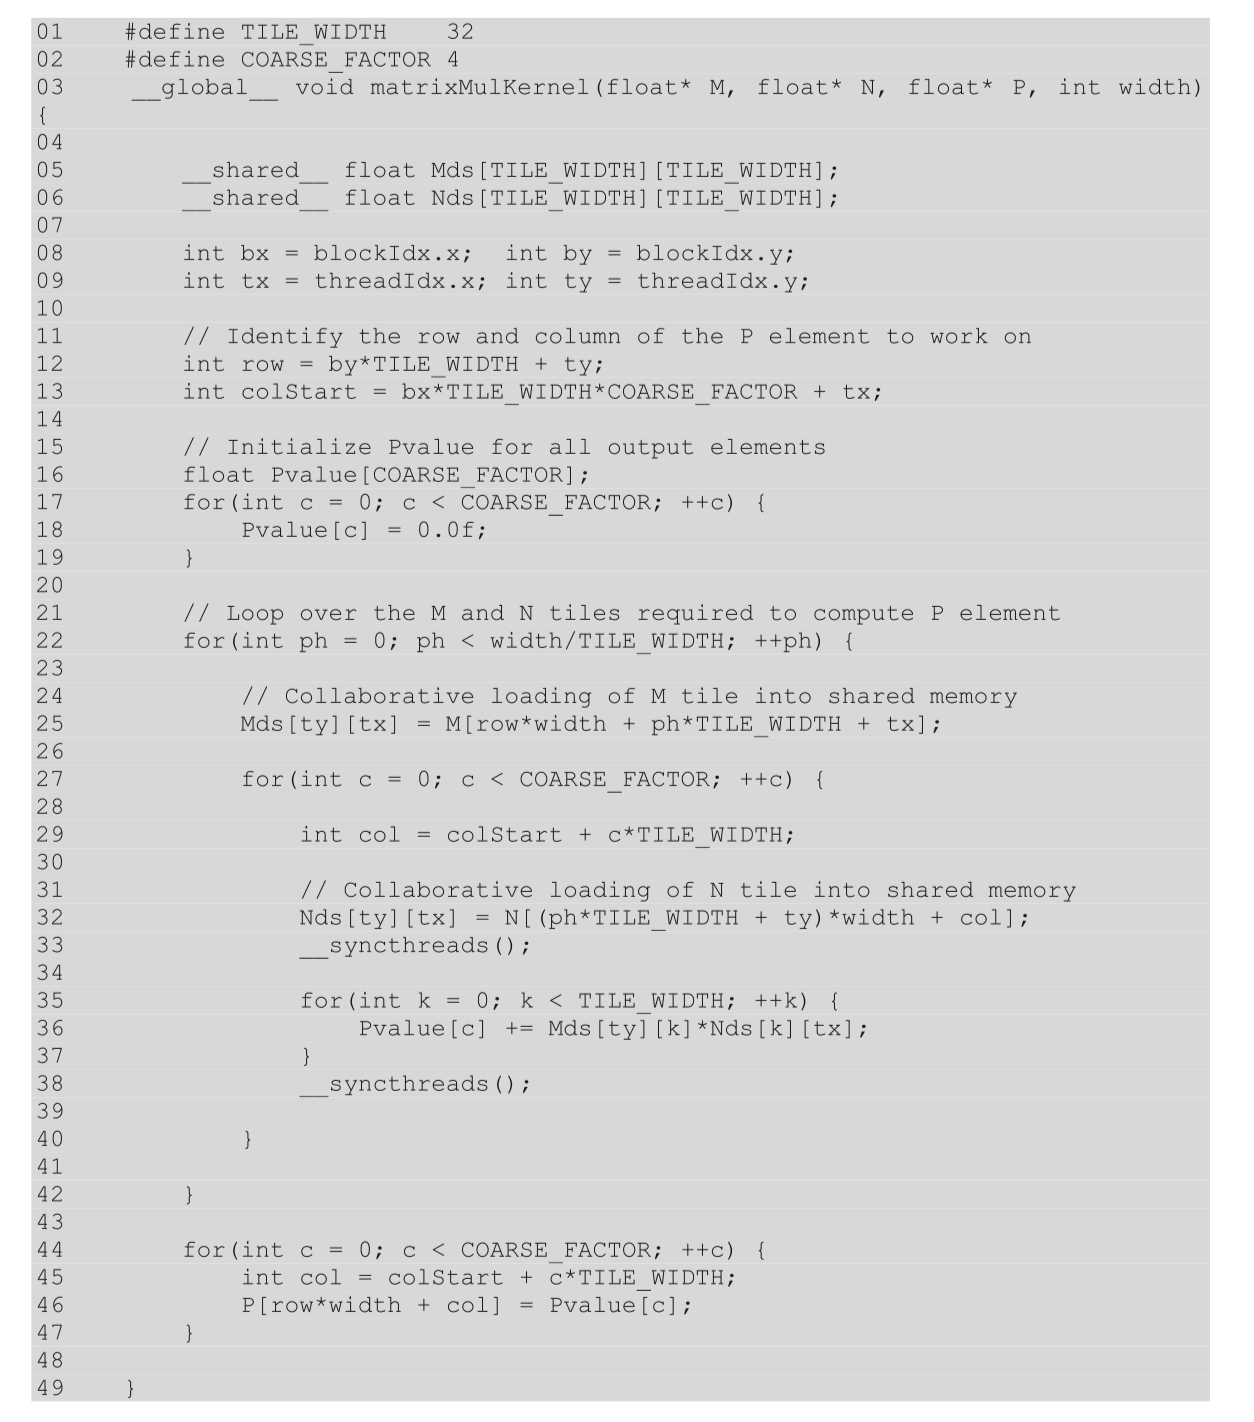
\includegraphics[width=0.9\textwidth]{figs/F6.13.png}
	\caption{\textit{用于平铺矩阵乘法的线程粗化的代码。}}
\end{figure}

图 6.13 显示了如何将线程粗化应用于第 5 章“内存架构和数据局部性”中的平铺矩阵乘法代码。 
在第 02 行添加了一个常量 COARSE\_FACTOR 来表示粗化因子,它是每个粗化线程将负责的原始工作单元的数量。 
在第 13 行,列索引的初始化被替换为 colStart 的初始化,它是线程负责的第一列的索引,
因为线程现在负责具有不同列索引的多个元素。 在计算 colStart 时,块索引 bx 乘以 TILE\_WIDTH → COARSE\_FACTOR,
而不仅仅是 TILE\_WIDTH,因为每个线程块现在负责 TILE\_WIDTH → COARSE\_FACTOR 列。 
在第 16-19 行,声明并初始化了 Pvalue 的多个实例,每个实例对应粗化线程负责的每个元素。 
第 17 行上的循环(迭代粗化线程负责的不同工作单元)有时称为粗化循环。 
在第 22 行循环输入图块的循环内,每次循环迭代中仅加载 M 的一个图块,与原始代码一样。 然而,对于加载的 M 个图块,
第 27 行的粗化循环会加载并使用 N 个图块。该循环首先找出粗化线程负责当前图块的哪一列(第 29 行),
然后 加载 N 的图块(第 32 行)并使用该图块来计算和更新每次迭代的不同 P 值(第 35-37 行)。 
最后,在第 44-47 行,每个粗化线程使用另一个粗化循环来更新它负责的输出元素。

线程粗化是一种强大的优化,可以显着提高许多应用程序的性能。 这是一种常用的优化。 
然而,在应用线程粗化时有几个需要避免的陷阱。 首先,必须小心不要在不必要时应用优化。 
回想一下,当并行化付出的代价可以通过粗化来降低时,例如数据的冗余加载、冗余工作、同步开销或其他,线程粗化是有益的。 
并非所有计算都有这样的价格。 例如,在第二章异构数据并行计算中的向量加法内核中,并行处理不同的向量元素是没有代价的。 
因此,将线程粗化应用于向量加法内核预计不会产生显着的性能差异。 
这同样适用于第 3 章“多维网格和数据”中的 RGB 到灰度转换内核。

要避免的第二个陷阱是不要应用太多粗化,以免硬件资源未得到充分利用。 
回想一下,向硬件提供尽可能多的并行性可以实现透明的可扩展性。 它为硬件提供了并行化或串行化工作的灵活性,
具体取决于硬件拥有的执行资源量。 当程序员粗化线程时,他们会减少暴露给硬件的并行量。 
如果粗化因子太高,则无法向硬件提供足够的并行性,从而导致一些并行执行资源未得到利用。 
在实践中,不同的设备具有不同数量的执行资源,因此最佳粗化因子通常是特定于设备和数据集的,
并且需要针对不同的设备和数据集重新调整。 因此,当应用线程粗化时,可伸缩性变得不太透明。

应用线程粗化的第三个陷阱是避免资源消耗增加到损害占用率的程度。 
根据内核的不同,线程粗化可能需要每个线程使用更多寄存器或每个线程块使用更多共享内存。 
如果是这种情况,程序员必须注意不要使用太多的寄存器或太多的共享内存,从而减少占用率。 
减少占用率带来的性能损失可能比线程粗化可能提供的性能优势更有害。

\subsection{优化清单}
在本书的第一部分中,我们介绍了 CUDA 程序员用来提高代码性能的各种常见优化。 
我们将这些优化整合到一个清单中,如表 6.1 所示。 该清单并不详尽,但它包含许多不同应用程序中常见的通用优化,
程序员应首先考虑这些优化。 在本书的第二部分和第三部分中,我们将把此清单中的优化应用于各种并行模式和应用程序,
以了解它们在不同上下文中的运行方式。 在本节中,我们将简要回顾每个优化及其应用策略。

\begin{figure}[H]
	\centering
	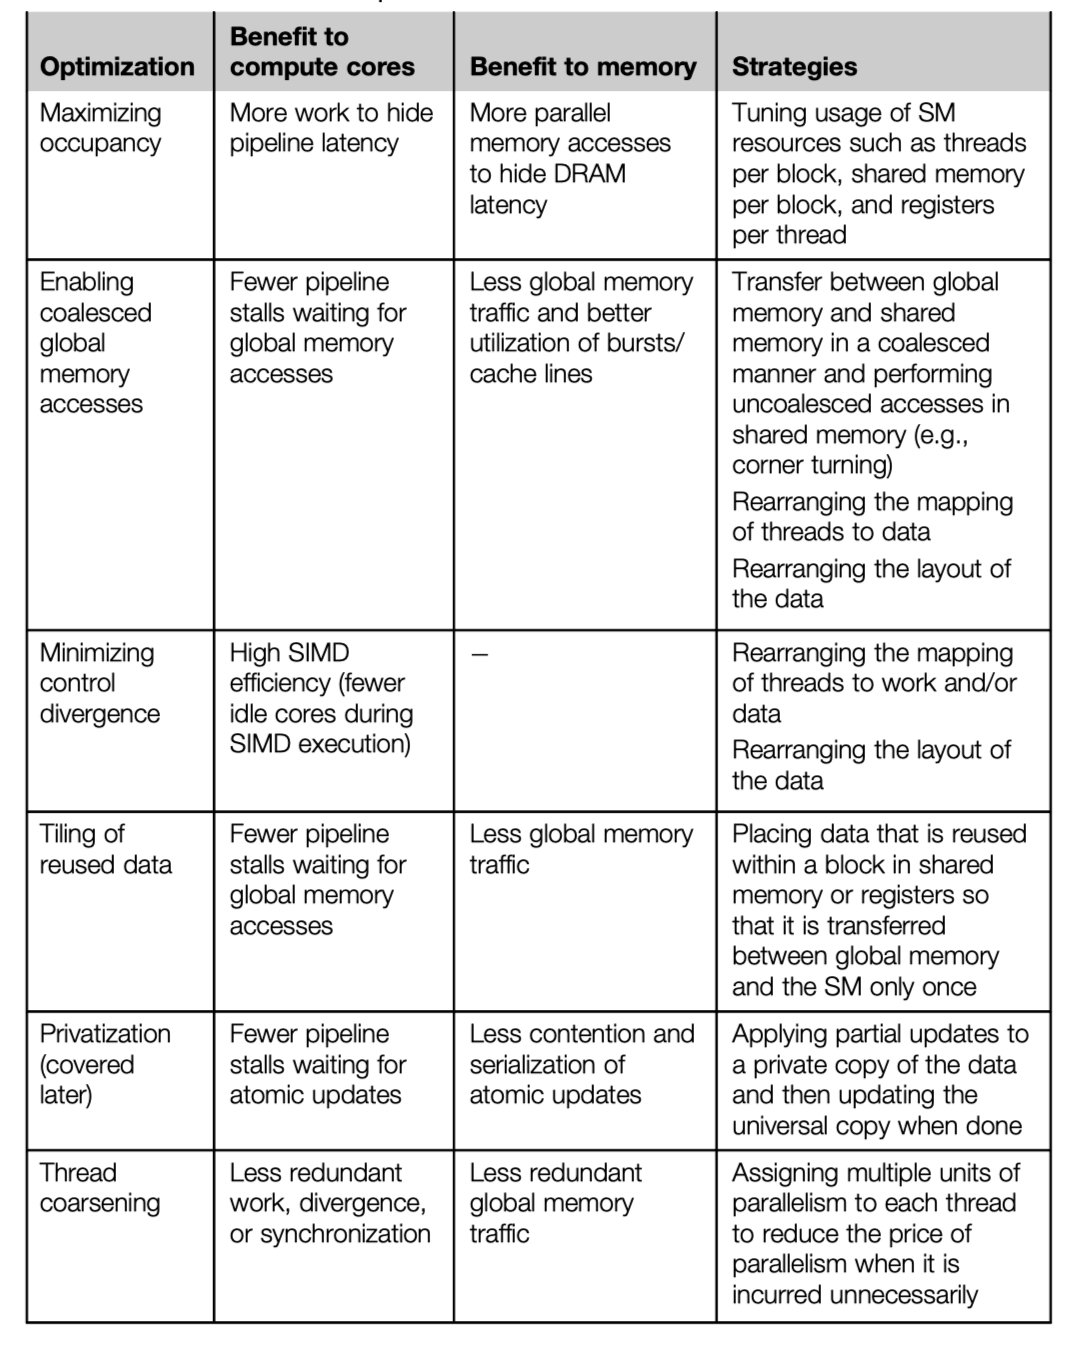
\includegraphics[width=0.9\textwidth]{figs/F6-a.2.png}
\end{figure}

表6.1中的第一个优化是最大化SM上线程的占用率。 这种优化在第 4 章“计算架构和调度”中介绍,
其中强调了拥有比内核多得多的线程的重要性,因为这是一种有足够的工作可用于隐藏核心管道中的长延迟操作的方法。 
为了最大限度地提高占用率,程序员可以调整其内核的资源使用情况,
以确保每个 SM 允许的块或寄存器的最大数量不会限制可以同时分配给 SM 的线程数量。 
在第 5 章“内存体系结构和数据局部性”中,引入了共享内存作为另一种资源,应仔细调整其使用,以免限制占用。 
在本章中,讨论了最大化占用率的重要性,作为隐藏内存延迟(而不仅仅是核心管道延迟)的一种手段。 
同时执行多个线程可确保生成足够的内存访问以充分利用内存带宽。

表 6.1 中的第二个优化是通过确保同一 warp 中的线程访问相邻内存位置来使用合并的全局内存访问。 
本章介绍了这种优化,其中强调了硬件将对相邻内存位置的访问组合成单个内存请求的能力,
作为减少全局内存流量和提高 DRAM 突发利用率的一种方法。 
到目前为止,我们在本书这一部分中看到的内核已经自然地展示了合并访问。 
然而,我们将在本书的第二部分和第三部分中看到许多示例,其中内存访问模式更加不规则,因此需要更多的努力来实现合并。

有多种策略可用于在具有不规则访问模式的应用程序中实现合并。 一种策略是以合并的方式将数据从全局内存加载到共享内存,
然后对共享内存进行不规则访问。 我们已经在本章中看到了这种策略的一个例子,即拐角。 
我们将在第 12 章“合并”中看到该策略的另一个示例,其中介绍了合并模式。 
在这种模式下,同一块中的线程需要在同一个数组中执行二分搜索,因此它们协作以合并的方式将该数组从全局内存加载到共享内存,
然后各自在共享内存中执行二分搜索。 我们还将在第 13 章“排序”中看到此策略的示例,其中介绍了排序模式。 
在此模式中,线程以分散的方式将结果写入数组,因此它们可以协作在共享内存中执行分散的访问,
然后将结果从共享内存写入全局内存,并为附近的元素启用更多合并 目的地。

在具有不规则访问模式的应用程序中实现合并的另一个策略是重新安排线程映射到数据元素的方式。 
我们将在第 10 章“归约和最小化分歧”中看到该策略的一个示例,其中介绍了归约模式。 
在具有不规则访问模式的应用程序中实现合并的另一个策略是重新安排数据本身的布局方式。 
我们将在第 14 章“稀疏矩阵计算”中看到该策略的一个示例,其中介绍了稀疏矩阵计算和存储格式,特别是在讨论 ELL 和 JDS 格式时。

表 6.1 中的第三个优化是最小化控制发散。 第 4 章“计算架构和调度”中介绍了控制发散,
其中强调了同一 warp 中的线程采用相同控制路径的重要性,作为确保在 SIMD 执行期间有效利用所有内核的方法。 
到目前为止,除了边界条件下不可避免的发散之外,我们在本书这一部分中看到的内核还没有表现出控制发散。 
然而,我们将在本书的第二部分和第三部分中看到许多例子,其中控制发散可能会严重损害性能。

有多种策略可以用来最小化控制发散。 一种策略是重新安排工作和/或数据在线程之间的分布方式,
以确保一个线程束中的线程在使用其他线程束中的线程之前全部使用。 
我们将在第 10 章“约化和最小化发散”(涵盖约化模式)和第 11 章“前缀和(扫描)”(涵盖扫描模式)中看到该策略的示例。 
重新安排工作和/或数据如何跨线程分布的策略也可用于确保同一线程束中的线程具有相似的工作负载。 
我们将在第 15 章“图遍历”中看到一个例子,其中介绍了图遍历,其中我们将讨论以顶点为中心和以边为中心的并行化方案之间的权衡。 
最小化控制分歧的另一个策略是重新安排数据的布局方式,以确保同一线程束中处理相邻数据的线程具有相似的工作负载。 
我们将在第 14 章“稀疏矩阵计算”中看到此策略的示例,其中涵盖稀疏矩阵计算和存储格式,特别是在讨论 JDS 格式时。

表 6.1 中的第四个优化是通过将块内重用的数据放置在共享内存或寄存器中并从那里重复访问它来平铺数据,
这样它只需要在全局内存和 SM 之间传输一次。 切片是在第 5 章“内存架构和数据局部性”中在矩阵乘法的背景下引入的,
其中处理相同输出切片的线程协作将相应的输入切片加载到共享内存,然后从共享内存重复访问这些输入切片 。 
我们将在本书的第二部分和第三部分中看到这种优化再次应用于大多数并行模式。 
当输入和输出图块具有不同尺寸时,我们将观察应用图块的挑战。 
这一挑战出现在第 7 章“卷积”(介绍了卷积模式)和第 8 章“模板”(介绍了模板模式)中。 
我们还将观察到数据块可以存储在寄存器中,而不仅仅是共享内存中。 
这一观察在第 8 章“模板”中最为明显,该章介绍了模板图案。 
我们还将观察到,平铺适用于重复访问的输出数据,而不仅仅是输入数据。

表6.1中的第五个优化是私有化。 此优化尚未介绍,但为了完整性我们在此提及。 
私有化涉及多个线程或块需要更新通用输出的情况。 
为了避免同时更新相同数据的开销,可以创建数据的私有副本并部分更新,然后在完成时从私有副本对通用副本进行最终更新。 
我们将在第 9 章“并行直方图”中看到这种优化的示例,其中介绍了直方图模式,其中多个线程需要更新相同的直方图计数器。 
我们还将在第 15 章“图遍历”中看到这种优化的示例,其中介绍了图遍历,其中多个线程需要向同一队列添加条目。

表 6.1 中的第六个优化是线程粗化,其中多个并行单元被分配给单个线程,以降低并行成本(如果硬件无论如何都要串行化线程)。 
本章在分片矩阵乘法的背景下介绍了线程粗化,其中并行性的代价是由处理相邻输出分片的多个线程块冗余地加载相同的输入分片。 
在这种情况下,分配一个线程块来处理多个相邻的输出图块使得能够为所有输出图块加载一次输入图块。 
在本书的第二部分和第三部分中,我们将看到线程粗化在不同的上下文中应用,每次都会有不同的并行性代价。 
在第 8 章“模板”中,介绍了模板图案,应用线程粗化来减少输入数据的冗余加载,如本章所示。 
在第 9 章“并行直方图”中,涵盖了直方图模式,线程粗化有助于减少在私有化优化的背景下需要提交到通用副本的私有副本的数量。 
在第 10 章“约化和最小化发散”(涵盖约化模式)和第 11 章“前缀和(扫描)”(涵盖扫描模式)中,
应用线程粗化来减少同步和控制发散带来的开销。 
同样在第 11 章“前缀和(扫描)”中,该章介绍了扫描模式,与顺序算法相比,线程粗化也有助于减少并行算法执行的冗余工作。 
在第 12 章“合并”中,介绍了合并模式,线程粗化减少了识别每个线程输入段所需执行的二分搜索操作的数量。 
第 13 章“排序”介绍了排序模式,线程粗化有助于改进内存合并。

同样,表 6.1 中的清单并非详尽无遗,但它包含不同计算模式中常见的主要优化类型。 
这些优化出现在本书第二部分和第三部分的多个章节中。 我们还将看到特定章节中出现的其他优化。 
例如,在第 7 章“卷积”中,介绍了卷积模式,我们将介绍常量内存的使用。 
在第 10 章“约化和最小化发散”中,涵盖了扫描模式,我们将介绍双缓冲优化。

\subsection{了解计算的瓶颈}
在决定对特定计算应用哪种优化时,首先要了解哪些资源限制了该计算的性能,这一点很重要。 
限制计算性能的资源通常称为性能瓶颈。 优化通常使用更多的一种资源来减轻另一种资源的负担。 
如果应用的优化不针对瓶颈资源,则优化可能不会带来任何好处。 更糟糕的是,优化尝试甚至可能会损害性能。

例如,共享内存平铺增加了共享内存的使用,以减轻全局内存带宽的压力。 
当瓶颈资源是全局内存带宽并且正在加载的数据被重用时,这种优化非常有用。 
然而,例如,如果性能受到占用的限制,而占用又受到使用过多共享内存的限制,那么应用共享内存平铺可能会使情况变得更糟。

为了了解哪些资源限制了计算性能,GPU 计算平台通常提供各种分析工具。 
我们建议读者参阅 CUDA 文档,以获取有关如何使用分析工具来识别计算性能瓶颈(NVIDIA、Profiler)的更多信息。 
性能瓶颈可能是特定于硬件的,这意味着相同的计算可能在不同的设备上遇到不同的瓶颈。 
因此,识别性能瓶颈和应用性能优化的过程需要充分了解 GPU 架构以及不同 GPU 设备之间的架构差异。

\subsection{总结}
在本章中,我们介绍了 GPU 的片外内存 (DRAM) 架构,并讨论了相关的性能注意事项,
例如全局内存访问合并和通过内存并行隐藏内存延迟。 然后我们提出了一个重要的优化:线程粒度粗化。 
通过本章和前面几章中介绍的见解,读者应该能够推断出他们遇到的任何内核代码的性能。 
我们通过提供广泛用于优化许多计算的常见性能优化清单来结束本书的这一部分。 
我们将在本书的接下来的两部分中继续研究这些优化在并行计算模式中的实际应用和应用案例研究。
